\documentclass[a4paper,10pt]{report}
\usepackage[utf8]{inputenc}
\usepackage{graphicx}
\usepackage{fullpage}
\usepackage{verbatim}
\usepackage[spanish]{babel}
\usepackage{wrapfig}
\usepackage{url}
\usepackage[font={scriptsize}]{caption}
\usepackage{makeidx}
\setcounter{secnumdepth}{3}
\setcounter{tocdepth}{3}
\makeindex

\selectlanguage{spanish}


\title{Implementación en GPU de un algoritmo eficiente de dinámica molecular con potenciales numéricos}
\author{Ignacio Eguinoa \\ 
\small Facultad de Informatica, UNLP
\date{}
}


\addtolength{\topmargin}{-35pt}
\addtolength{\textwidth}{80pt}
\addtolength{\textheight}{100pt}
\addtolength{\oddsidemargin}{-40pt}


\begin{document}

\maketitle



\section*{Resumen} 



En este trabajo se presenta una optimizacion del algoritmo de dinamica molecular sobre GPU para simulacion de sistemas de particulas que interaccionan mediante un potencial de Lennard-Jones. 

Siguiendo las especificaciones del método de dinámica molecular se desarrolla, en primer lugar, una implementacion propia de éste sobre GPU que evoluciona exlusivamente de acuerdo a un modelo de potencial de Lennard-Jones. Usando este desarrollo como referencia, se implementan adaptaciones para el calculo del potencial y las fuerzas derivadas de éste basadas en el uso de valores tabulados, teniendo en cuenta tanto las propiedades de la funcion potencial como las caracteristicas del hardware sobre el cual se trabaja.

Además de las mejoras en performance, se tiene en cuenta otro aspecto importante: la precisión numérica con la que se opera. Dado que la utilización de valores tabulados implica un error en el potencial y su fuerza resultante, es necesario evaluar la implicancia que tendrá esto sobre la correctitud de la simulación.

Las implementaciones actuales del método sobre arquitecturas GPU proveen una gran mejora en la performance con respecto a las versiones iniciales implementadas sobre CPU, lo cual es producto de las propiedades intrínsecamente paralelas del algoritmo y la arquitectura altamente paralelizada del hardware. Por su parte, las adaptaciones realizadas en este trabajo presentan una optimizacion extra manteniendo la calidad númerica de los resultados. 

Dado que el potencial de Lennard-Jones representa un aporte importante para modelar las interacciones en distintos campos de fuerzas, las mejoras obtenidas pueden ser incorporadas fácilmente a distintas versiones existentes del método de dinámica molecular. 

Por último, los resultados obtenidos alientan a evaluar este tipo de aproximaciones para realizar cálculos con formas funcionales similares que hayan sido implementados sobre GPU. De esta forma, se intenta explotar todas las propiedades que ofrece la arquitectura.


\pagebreak




\tableofcontents

\pagebreak


\chapter{Introducción}


\section{Objetivos}



El principal objetivo de la tesis es obtener una implementacion del método de dinámica molecular basada en GPU, que siga un modelo de interaccion de 
Lennard-Jones(potencial de no-union), y que resuelva el calculo de las fuerzas utilizando valores tabulados en el sistema de memoria provisto por la arquitectura. 

La forma funcional que describe el potencial de Lennard-Jones permitiria obtener una buena aproximación del valor utilizando una tabla de resultados precalculados. 
Además, el sistema de memorias de la arquitectura, que ha evolucionado considerablemente desde su creación de esta, permite recuperar de forma eficiente el valor asociado en un esquema de tablas. 
De esta forma, se espera que la modificacion resulte en una mejora de la performance manteniendo la correctitud en los resultados de la simulación. 



\section{El metodo de dinamica molecular}

\subsection{Fundamentos}


Los sistemas químicos de interés como las proteínas suelen ser complejos de estudiar debido a su gran tamaño. 
La superficie de energia libre es la funcion que describe la energia del sistema, y a partir de la cual se podrian
derivar todas las propiedades termodinamicas y cineticas de interes. Esta, sin embargo, es una funcion 3N dimensional (siendo N el numero de particulas del sistema), lo que hace imposible derivar analiticamente las propiedades debido al altisimo costo computacional asociado.
Otra forma de analizar estos sistemas es mediante una aproximación numérica, a través de simulaciones computacionales.  	

La simulación computacional de biomoléculas involucra la exploración de su superficie de energía libre, la cual, debido a la complejidad de estos sistemas, es altamente accidentada, contiene una gran cantidad de mínimos locales y de barreras de energéticas. 
De esta forma, si los parametros de la simulacion estan correctamente definidos, el conjunto de conformaciones adoptadas durante la ejecucion sera representativo del ensamble real de conformaciones posibles del sistema, lo que nos permite estimar las propiedades de interes.
Los métodos de simulación molecular nos permiten, entonces, obtener una serie de configuraciones representativas del sistema, de modo que las propiedades termodinámicas extraídas del mismo se correspondan de manera precisa con los valores reales.
Una de las formas de obtener estas configuraciones es mediante el metodo de dinamica molecular. Este metodo implica simular la progresion temporal "real" del sistema, obteniendo distintas conformaciones a medida que avanza el tiempo de simulacion.

La tecnica de simulacion de Dinamica Molecular se basa en resolver las ecuaciones de movimiento de Newton para cada átomo del sistema; así, en cada "paso" de la simulación se calcula la energia potencial entre las particulas y de esta se derivan las fuerzas que actúan sobre cada átomo. 
Las ecuaciones de Newton relacionan las fuerzas resultantes del potencial con la aceleracion que tendra cada particula y, por lo tanto, el cambio en la velocidad y en la posicion con el tiempo. 
Dado que el potencial es una funcion continua dependiente de la posicion, los cambios en las velocidades y posiciones resultan de una integracion a lo largo de la trayectoria de la particula.


\subsection{Esquema general del método}

En la practica, la integración de las Ecuaciones de Newton se calcula computacionalmente mediante el llamado Algoritmo de Verlet [14], el cual resuelve la integración en una ecuacion discreta donde las posiciones estan separadas por intervalos de tiempo ("dt") . 
Usando las fuerzas resultantes, junto con las posiciones y velocidades de las particulas correspondientes a la iteracion, el algoritmo de Verlet calcula las nuevas posiciones y velocidades en un intervalo de tiempo posterior. De este modo se genera una trayectoria, determinada por las posiciones de las particulas en cada paso de la simulacion. Esta trayectoria describe como cambia la conformación espacial del sistema a lo largo del tiempo. 
La elección del ''dt'' es una situación de compromiso, ya que un valor muy chico, si bien representa la propagación del movimiento de forma mas precisa(mas cercana al valor de la integracion), requiere una mayor cantidad de cálculos para un mismo tiempo total de simulación. 



El esquema general del método es el siguiente:


% \begin{figure}[!ht]
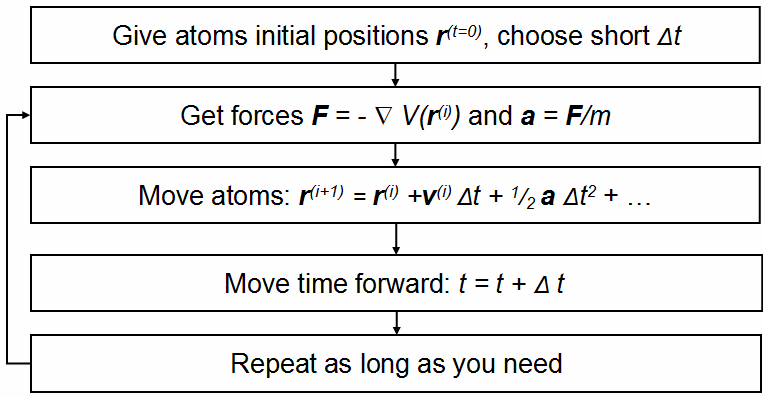
\includegraphics[keepaspectratio, width=\textwidth]{img/mdalgorithm.png}
% \caption{Esquema general del algoritmo de dinámica molecular}
% \label{Fig:esquemaMD}
% \end{figure}

% ***************CAMBIAR LA FIGURA POR UNA SIMILAR EN ESPAÑOL **********
% \linebreak

\vspace{20pt}



% *********************
% ****QUE OTROS DATOS RELEVANTES OBTENGO DE LA SIMULACION??
%********************** 
  



El resultado de una simulación de dinámica molecular es principalmente una trayectoria representada por la posición de cada una de las particulas a lo largo de un cierto tiempo.
No se va a detallar acerca de los metodos para el procesamiento de este resultado pero es relevante decir que la longitud de trayectoria que podamos obtener en un tiempo de cómputo razonable es lo que limita el tipo de proceso químico que podremos estudiar.
Para poder estudiar un cierto proceso de interés es necesario que la simulacion alcance la escala de tiempo en la cual este ocurre. Un mayor tiempo de simulación equivale a realizar mas pasos y por lo tanto mas calculos totales, aumentando asi el tiempo de computo requerido.

Por su parte, simular sistemas mas grandes (con mayor cantidad de particulas) implica una mayor cantidad de calculos en cada paso y por lo tanto un mayor costo computacional. Además, la funcion que describe las propiedades del sistema tiene por naturaleza una mayor cantidad de variables, debido a esto es necesario  correr la simulacion durante mas tiempo para poder llegar a un conjunto de conformaciones que sea representativo del ensamble real.





\subsection{La función potencial}


En la utilización del método de dinámica molecular, el potencial(V) que permite derivar las fuerzas entre particulas se obtiene modelando al sistema molecular mediante la mecanica clasica (metodo de mecanica molecular, MM).
Usando un método de MM [12] , se ignoran los electrones y la naturaleza cuántica de estos. La energía potencial del sistema, entonces, depende exclusivamente de las posiciones de los núcleos atómicos. Se modela cada molécula como un conjunto de sitios -que representan los átomos que la componen- y resortes -que representan los enlaces químicos entre estos- junto con un potencial parametrizado ad hoc.
Este potencial es una función matemática que depende exclusivamente de las posiciones de los atomos, intentando ajustarse a las interacciones entre los componentes del sistema sistema real. Este tipo de repesentacion simplificada del sistema permite reducir la complejidad de los calculos necesarios para la simulacion, y por lo tanto el costo computacional asociado, pero limita el tipo de procesos que se pueden estudiar. Por ej. no se pueden estudiar reacciones quimicas que impliquen ruptura o formación de enlaces ya que estos no son considerados con suficiente detalle.

% The choice of the molecular mechanics force fields is an important aspect of the MD simulation . The forcefield governs how the parts of a molecule relate to each other, how each atom is affected by its atomic environment and how these forces can contribute to the structure of the molecule under a certain set of constraints
Las interacciones representadas en el método de MM se pueden agrupar en dos tipos:

\begin{description}
 \item [De unión:] Describen las interacciones entre dos átomos unidos entre si directamente o hasta 2 enlaces de distancia. Consisten en aquellos términos del potencial cuya energía se ve afectada por los
estiramientos de los enlaces, las flexiones de los ángulos entre 2 átomos, y la rotación de dos átomos adyacentes sobre un eje (ángulos dihedros). Los estiramientos y las flexiones angulares son modeladas
mediante un oscilador armónico, mientras que las rotaciones de los enlaces en el plano son modeladas mediante una función trigonométrica.

\item [De no unión:] describen la interacción entre átomos ubicados a más de 3 enlaces de distancia de la
misma molécula, o bien entre átomos de moléculas distintas, y consisten en un término para la
contribución electrostática computada con la Ley de Coulomb, y un término para la contribución de
Vaan Der Waals modelada por un potencial de Leenard-Jones 12-6.


\end{description}



El esquema general de la función potencial suele tomar una forma similar a la que sigue: \\ \\ 
% ***PONER la funcion que marca la diferencia entre los parametros de union y los de no union PAGINA 15 DE LA TESIS***
% 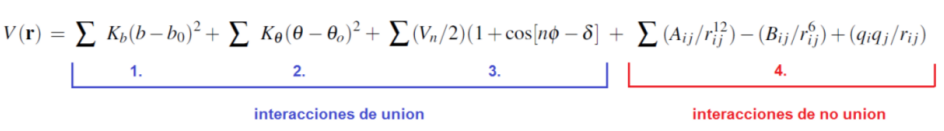
\includegraphics[]{img/ecPotencialAmber.png}
% \begin{figure}[h]
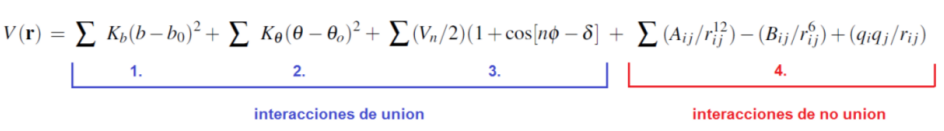
\includegraphics[keepaspectratio, width=1.0\textwidth]{img/ecPotencialAmber.png}
% \caption{Ejemplo de potencial de interacción del paquete de software Amber}
% \label{Fig:Amber}
% \end{figure}
\vspace{2pt}

En azul se representan los términos matemáticos que modelan las interacciones de unión (1. Término de estiramiento de enlaces; 2. Término de flexión angular; 3. Término de rotación de ángulos diedros), y en rojo
las interacciones de no unión (Potencial de Leenard-Jones 12-6 e interacción Coulómbica).

Los parámetros que se observan en esta función potencial (las constantes $K_b, K_{\theta}$ y $V_n$ , los valores de equilibrio $b_0$, $\theta_0$ y $\delta$ , 
las constantes A y B correspondientes al potencial Lenard-Jones, y las cargas q) deben ser ajustados especialmente para cada molécula individual que se desee incluir en la 
simulación. Estos parámetros se suelen obtener tanto de datos experimentales, como así también de rigurosos cálculos cuanticos, y en ocasiones emplean correcciones empíricas.
Al conjunto o "set" de parámetros derivados para utilizarse de forma conjunta en una simulación se lo conoce como Campo de Fuerzas.

% *************************
% ********ACA DEBERIA HABLAR DE LOS DISTINTOS CAMPOS DE FUERZAS QUE EXISTEN, QUE GENERAN DIFERENTES VERSIONES DEL ALGORITMO, LOS CUALES PUEDEN SER  MAS GENERALES O APUNTAR A DISTINTOS TIPOS DE SISTEMAS
% ******************************


El modelo de interaccion(campo de fuerzas) es la principal diferencia entre los distintos paquetes de software para simulaciones de dinamica molecular.
Este campo de fuerzas esta parametrizado especificamente para el tipo de sistema que se intenta simular, de forma que se ajuste lo mejor posible a la realidad. De esta forma, existen versiones especificas para simular sistemas biologicos (proteinas, acidos nucleicos), otros que intentan abarcar a sistemas de quimica organica en general, etc.




\subsubsection{Potencial de Lennard-Jones}


El calculo del potencial de no union es una parte importante en la implementacion del algoritmo ya que implica la mayor parte del costo computacional asociado a la simulacion. 
Esto se debe a que se debe calcular entre todos los elementos del sistema. 
En particular, es importante el termino correspondiente al potencial de Lennard-Jones porque este existe siempre, independientemente de la carga neta en las particulas que interaccionan.

La ecuacion que representa este potencial es:


% TENGO QUE EXPLICAR QUE LOS PARAMETROS SIGMA Y EPSILON DEPENDEN DE LOS TIPOS DE PARTICULAS QUE ESTAN INTERACTUANDO, ES IMPORTANTE DEJARLO CLARO PORQUE ES RELEVANTE PARA LA IMPLEMENTACION DEL ALGORITMO YA QUE VOY A NECESITAR MATRICES CON LOS VALORES PARA TODAS LAS COMBINACIONES DE TIPOS DE ELEMENTOS

La forma funcional de esta interaccion resulta: 
% ****PONER GRAFICO DEL POTENCIAL vs DISTANCIA

A partir de los valores del grafico, resulta razonable pensar que, si se desprecia el aporte de este potencial para interacciones entre particulas a una distancia mayor que cierto valor de corte, se podra obtener una buena aproximacion del comportamiento a la vez que se reduce considerablemente la cantidad de calculos necesarios en cada paso de la simulacion.


\begin{comment}
***************LA INTRODUCCION PUEDE TERMINAR ACA, APUNTANDO AL POTENCIAL DE LENNARD-JONES, O PUEDE INCLUIR TAMBIEN LO QUE SIGUE*********

*********************ESTO QUE SIGUE PUEDE IR DIRECTAMENTE EN LA PARTE DE ALGORITMOS ***************************
*******HABLA DE LA DIVERSIDAD DE VARIANTES QUE EXISTEN, Y ALGO DE LAS OPTIMIZACIONES DEL ALGORITMO (OPTIMIZACIONES RELACIONADAS CON EL METODO EN SI Y VARIACIONES EN LOS CALCULOS QUE HAY QUE HACER)*******

*****PUEDO ARRANCAR EXPLICANDO POR QUE ES NECESARIO OPTIMIZAR EL METODO PARA PODER EJECUTAR MAS TIEMPO. TENGO QUE OPTIMIZARLO PARA REALIZAR EJECUCIONES MAS EFICIENTEMENTE Y PARA PODER AMPLIAR LA UTILIZACION DEL METODO PARA SIMULAR SISTEMAS MAS GRANDES Y DURANTE MAS TIEMPO, PARA PODER APLICARLO A OTROS SISTEMAS Y PROCESOS DE INTERES***
\end{comment}


Como se mencionó previamente, el potencial de L-J es uno de los componentes que se encuentra en la mayoria los campos de fuerza existentes, por lo que optimizar el calculo de este tendria una gran ventaja. 
Ademas, al ser una interaccion de no union, existe, al menos debilmente, entre todos los pares de particulas del sistema, lo que implica una gran cantidad de calculos por paso. El calculo de potenciales de no union representa asi la mayor parte del costo computacional asociado a la simulacion, existen algunas optimizaciones para el calculo del aporte electroestatico pero no para el componente de L-J de manera que este genera un cuello de botella en las mejoras del tiempo de ejecucion.





% **********************************************************
% ************** EXPLICAR CONDICIONES DE PERIODICIDAD
% *************************************************************
\subsection{Condiciones de periodicidad}


Real systems are almost infinite in size

In vacuo simulation are rarely a good idea

Periodic boundary conditions: 
-Simulation boxes and nearest image conventions

-Infinite electrostatics: Ewald summation

-Problem: physical properties depend on box size







% *-**********************************************
%***   PODRIA AGREGAR UNA subsection DEDICADA AL ESTADO DEL ARTE( O  CON OTRO NOMBRE) , DONDE HABLE DE:
%   -PODRIA ARRANCAR DICIENDO QUE EL METODO HA EVOLUCIONADO MUCHO, IMPUSADO POR LA GRAN UTILIDAD DE ESTE 
%   -DISTINTAS OPTIMIZACIONES EN EL METODO (VARIACIONES EN LA FORMA DE IMPLEMENTAR LA INTERACCION CON EL SOLVENTE ...PME, SOLVENTE IMPLICITO, ETC)
%  
%  -NO DEBERIA HABLAR DE IMPLEMENTACIONES EN SI (PARALELA, GPUS, ETC), SOLO DE CUESTIONES RELACIONADAS CON EL METODO EN SI MISMO. 
%        ******PERO SI PODRIA HABLAR DE QUE EL METODO PERMITE DIFERENTES IMPLEMENTACIONES Y LOS AVANCES EN EL HARDWARE Y MODELOS DE COMPUTO HAN GENERADO UNA GRAN VARIEDAD DE IMPLEMENTACIONES
%  -CUALES SON LOS ORDENES DE TIEMPO DE SIMULACION DE INTERES Y CUALES LOS QUE SON MANEJABLES CON EL EQUIPAMIENTO DE HOY EN DIA. 
%  -LO MISMO CON RESPECTO A LOS TAMAÑOS DE LOS SISTEMAS DE PARTICULAS
%  -DEBERIA DECIR QUE HAY MUCHOS PROCESOS QUE OCURREN EN ESCALAS DE TIEMPO QUE NO SE PUEDEN MANEJAR TODAVIA Y POR LO TANTO SE CONTINUA INTENTANDO MEJORAR LOS TIEMPOS DE SIMULACION
%************************************************



\subsection{Estado del arte}


Existen distintas aproximaciones para evaluar las interacciones que apuntan a optimizar el costo computacional asociado al calculo. Algunas implementaciones permiten definir un potencial de solvente implicito, ...... (referencia : Born solvation model [V. Tsui  D.A. Case, Biopolymers (Nucl. Acid. Sci.) 56, 275-291 (2001)].)
Otra optimizacion posible es para el calculo del potencial de interaccion electrostatico : PME. Este es importante ya que permite simplificar el calculo del aporte electroestatico el cual, al ser un potencial de no-union, implica una gran cantidad de calculos.






En cuanto a las arquitecturas de cómputo, las implementaciones sobre GPU, que son el centro de este trabajo, se han establecido como estándares para las implementaciones del algoritmo. Esto se debe 


Con este contexto , las capacidades de cálculo actuales permiten realizar simulaciones de dinámica molecular en sistemas de hasta XXXXXXXXXX átomos aproximadamente sobre un intervalo de tiempo del orden de YYYYYYY  micro/pico/******segundos).

Si bien se ha avanzado mucho desde el desarrollo del método, existen multiples procesos de interes que podrían ser abordados mediante experimentos de simulacion computacional pero que el intervalo de tiempo en el cual ocurren no es posible de ser alcanzado con los recursos disponibles hoy en dia.
Esta situación hace que se destine una gran cantidad de esfuerzo para continuar las mejoras en el metodo y mantener las implementaciones a la par de las arquitecturas disponibles.





\chapter{La arquitectura GPU}





\chapter{Algoritmos}
\begin{comment}
 
PRIMERO HAY UNA PARTE GENERAL DE ´INTRODUCCION´:  EN ESTA PARTE TENGO QUE ACLARAR BIEN LOS FUNDAMENTOS DE LA MODIFICACION 
-EN PRIMER LUGAR TENGO QUE EXPLICAR QUE ES LO QUE YA EXISTE EN CUANTO A IMPLEMENTACIONES DE DINAMICA MOLECULAR (AMBER GPU, ETC). P 
PUEDO ARRANCAR ´ASUMIENDO´ QUE LA IMPLEMENTACION SECUENCIAL ES CASI OBVIA Y DIRECTA A PARTIR DE LA ESPECIFICACION QUE SE DIO EN LA INTRODUCCION.
VOY PLANTEANDO TODAS LAS OPTIMIZACIONES QUE SE FUERON HICIENDO(APROVECHANDO AVANCES EN LAS ARQUITECTURAS/MODELOS DE COMPUTO). EN LA INTRODUCCION YA HABLE DE OPTIMIZACIONES REFERIDAS AL METODO EN SI MISMO Y TERMINE DICIENDO QUE LA PARTE DE L-J ES LA QUE MAS CUESTA Y LA QUE MENOS OPTIMIZACIONES TIENE.
-DESPUES EXPLICO POR QUE SE PUEDE PENSAR QUE USANDO LA GPU (Y ASUMIENDO LA IMPLEMENTACION SOBRE GPU COMO BASE) PUEDO USAR UNA TABLA PARA BUSCAR LOS RESULTADOS DE LA FUNCION (POTENCIAL L-J). ACA PUEDO DECIR QUE LA TABLA PUEDE SER IMPLEMENTADA EN CUALQUIER SISTEMA DE MEMORIA. ES DEICR, SI BIEN SE PUEDE IMPLEMENTAR SOBRE CPU ESTA SOLUCION (Y DE HECHO LO HICE) USAMOS LA GPU POR LA MEMORIA DE TEXTURA Y POR SER HOY EN DIA UN ESTANDAR EN LO QUE RESPECTA A DINAMICA MOLECULAR

DESPUES DE LA INTRODUCCION ARMO UNA SECCION (3.1, 3.2, etc) PARA CADA UNA DE LAS VARIANTES. AHI DETALLO CADA VARIANTE:
SOLO ARMO 3 SECCIONES: EL ALGORITMO BASE DONDE EXPLICO TODO, EL ALGORITMO QUE USA UNA TABLA CON EL POTENCIAL, Y EL ALGORITMO QUE USA UNA TABLA CON EL VALOR DE LAS DERIVADAS.
DESCRIBO LOS ALGORITMOS IMPLEMENTADOS, AGREGANDO CUALQUIER DETALLE QUE HAGA FALTA (QUE NO ESTE EN LA INTRODUCCION DE DINAMICA MOL.).
LA PARTE DE PERIODICIDAD LA EXPLICO ACA???


****
TENGO UNA LINEA ACA QUE TRAJE DE OTRO LADO, NO SE DONDE METERLA:
Existen diversas implementaciones del algoritmo de dinamica molecular con diferentes modelos de interaccion. Las distintas implementaciones existentes involucran al potencial de Lennard-Jones como aporte para evaluar las interacciones de no-union y, en todos los casos, el calculo de este tipo de interacciones representa la mayor parte del costo computacional asociado al método. Se espera entonces que las modificaciones estudiadas en este trabajo puedan ser integradas en diversas implementaciones existentes obteniendo una mejora considerable en la performance.
*****

\end{comment}




% ***ESTE PRIMER PARRAFO QUE DICE QUE LAS IMPLEMENTACIONES SOBRE GPU SON UN ESTANDAR ....*****LO SAQUE DE LA PARTE DE OBJETIVOS**


A partir de la descripción del método presentada en el capitulo 1 se puede llegar a una implementacion secuencial en forma casi directa. Este tipo de versiones son las que se utilizaron inicialmente para realizar las simulaciones.
La utilidad que ha mostrado esta técnica desde sus inicios y la posibilidad que ofrece para nuevas aplicaciones hizo que se desarrollen diversas implementaciones para aprovechar los nuevos modelos de computo disponibles, los cuales han avanzado considerablemente teniendo en cuenta que la tecnica fue creada hace ya un largo tiempo. 
Entre los nuevos algoritmos, una gran cantidad se ha enfocado en explotar las caracteristicas intrinsecamente paralelas del metodo. En los ultimos años, con avance de las arquitecturas de GPU y su utilizacion para computo de proposito general, estos algoritmos han sido portados para adaptarse a las caracteristicas propias de GPGPU.
De las versiones mencionadas en el capitulo 1, gran parte de ellas han sido portadas para poder ejecutarse sobre estas arquitecturas. (referencias amberGPU?? gromacs gpu??).

En el capitulo anterior se mostraron las ventajas que brinda el metodo de GPGPU para aplicaciones altamente paralelizables. De la misma forma,  la implementacion del metodo de dinamica molecular sobre esta arquitectura resulta en un aumento muy importante en la performance en forma casi directa. Además de las mejoras en la performance, el bajo costo del hardware en relacion a su poder de computo que provee la arquitectura hace que estas implementaciones sean un estandar de uso en el area.  

De esta forma, hoy en dia se puede encontrar una gran variedad de software para simulaciones de dinamica molecular implementado sobre GPU. A pesar de la gran cantidad de modificaciones que se han agregado y la evolucion en el hardware existente, se sigue dedicando un gran esfuerzo para continuar optimizando el algoritmo con el fin de poder simular nuevos procesos y sistemas de interes que requieren una mayor cantidad de calculos. 
Si se analizan las implementaciones que se utilizan actualmente, se puede ver que la mayor parte del costo computacional del metodo se mantiene asociado al calculo de las interacciones de no-union(entre particulas que no forman enlaces quimicos entre si), el cual esta representado principalmente por el potencial de L-J. Este calculo tiene una complejidad de orden N2 sobre el numero de particulas del sistema....
En el capitulo 1 se describio una aproximacion muy utilizada para intentar reducir la cantidad de calculos necesarios, la cual consiste en despreciar las interacciones entre particulas que se encuentren a mayor distancia que cierto valor de cutoff. Esta aproximacion esta basada en las propiedades de la funcion que describe el potencial de L-J. Incluso ajustando el valor de cutoff a valores suficientemente chicos, el costo que implica este paso representa la mayor parte de los requerimiento......Por esta razon, una gran parte de los esfuerzos se centran en optimizar esta etapa.
 

% ****HASTA ACA YA DEFINI QUE LAS IMPLEMENTACIONES SOBRE GPU SON EL ESTANDAR HOY EN DIA, Y QUE SE HA OPTIMIZADO POCO DEL CALCULO DEL POTENCIAL DE LENNARD-JONES PERO SI DE OTROS ASPECTOS, INCLUSO SE HA OPTIMIZADO EL CALCULO DE LAS INTERACCIONES ELECTROSTATICAS***

% ****AHORA EXPLICO CUALES SON LAS CARACTERISTICAS DE LA FUNCION DE L-J QUE HACEN QUE PUEDA SER TABULADO Y DAR UNA BUENA APROXIMACION 
% DESPUES EXPLICO QUE LAS CARACTERISTICAS DE LA MEMORIA DE TEXTURA ENCAJAN JUSTO PARA IMPLEMENTAR LA TABLA Y LA BUSQUEDA EFICIENTE DEL RESULTADO ASOCIADO***


Como se puede apreciar a partir de la descripcion de este potencial en el capitulo 1, la forma funcional que lo describe se caracteriza por tener un rango de distancias donde el resultado crece(o decrece) exponencialmente, y un punto a partir del cual converge y el valor asociado a la interaccion se hace despreciable.
Basandose en estas caracteristicas es razonable pensar que, utilizando una tabla conteniendo los resultados para un rango de valores definido y, aun sin tener ésta un tamaño excesivo, se podria obtener una buena aproximacion del resultado para cualquier distancia. 


% ****ACA PONGO LAS CARACTERISTICAS QUE OFRECE LA GPU Y QUE PUEDEN SER USADAS APROVECHANDO QUE HOY EN DIA LA MAYORIA DEL SOFT. ESTA IMPLEMENTADO SOBRE GPU*****

Para implementar este mecanismo hay varias propiedades del sistema de memoria que se puede usar y que se deben analizar......................................................



% ****ALGO MAS ANTES DE TERMINAR***

Se debe tener en cuenta que, aún cuando sea posible realizar una buena aproximacion utilizando tablas, el algoritmo de dinamica molecular implica utilizar este valor para obtener las fuerzas y movimientos resultantes de la interaccion, lo cual afecta la posicion (y por lo tanto el valor del potencial asociado) en la proxima iteracion. De esta forma, los errores resultantes de la aproximacion por utilizar tablas de valores seran propagados a lo largo de una simulacion que involucra miles de pasos.....


% ****TERMINO CON****

Asi, en este trabajo se estudiarán distintas formas de utilizar el sistema de memoria de la gpu para realizar el calculo del potencial de Lennard Jones, analizando su utilizacion en el contexto del método de dinamica molecular. Dado que el calculo de este potencial representa la mayor parte del costo asociado a la simulacion, se espera obtener una mejora considerable en el tiempo de ejecución con respecto al algoritmo estandar sobre GPU, el cual resuelve la ecuacion de L-J para cada interaccion a evaluar.




\begin{comment}

**********************************
EN ESTAS SECCIONES DEBERIA HACER UNA DESCRIPCION GENERAL DE LOS 3 ESQUEMAS QUE DESARROLLO(DESPUES CADA UNO PUEDE LLEVAR A 1 O MAS IMPLEMENTACIONES Y VARIANTES).  
-EN EL ALGORITMO QUE USA LA TABLA DEL POTENCIAL SIMPLEMENTE PONGO QUE USO UNA TABLA DONDE POR CADA VALOR DE DISTANCIA TENGO ASOCIADO UN VALOR, QUE A PARTIR DE AHI TENGO QUE AGARRAR 2 VALORES DE LA TABLA PARA PODER OBTENER LA DERIVADA, PUEDO AGREGAR QUE LA VENTAJA DE TENER TABULADO EL VALOR DEL POTENCIAL ES QUE SI QUIERO CALCULAR EL POTENCIAL TOTAL SOLO TENGO QUE LEER 1 DATO DE LA TABLA....BLA BLA.....NO MUCHO MAS.
-EN LA OTRA VERSION, DONDE TENGO TABULADA LA DERIVADA, TENGO QUE EXPLICAR PRIMERO POR QUE NECESITO LA DERIVADA (SUPUESTAMENTE ESTO YA TIENE QUE ESTAR BASTANTE CLARO), 
\end{comment}







\section{Algoritmo base sobre GPU (o Esquema general del algoritmo)}


% ***PUEDO ARRANCAR DE UNA EXPLICANDO EL ALGORITMO Y DESPUES COMENTO LA VENTAJA DE TENER ESTA IMPLEMENTACION ****


El algoritmo inicial sigue la especificacion que se detallo en el capitulo 1....
Dado que el aporte al campo de fuerzas que nos interesa es el correspondiente al potencial de L-J (potencial de no union), este es el unico aporte que se va a considerar. De esta forma, el sistema evoluciona en el tiempo a partir de las velocidades iniciales de las particulas y las fuerzas que se derivan de este potencial, unicamente. Si bien este modelo (considerando solo la interaccion de L-J) no es de utilidad para simular sistemas biologicos de interes (donde existen diversos enlaces entre los elementos), en este caso 



Si bien el codigo aqui implementado ya está implementado como parte de distintos paquetes de software de dinamica molecular, el objetivo de realizar un algoritmo independiente, donde la evolucion temporal ocurra unicamente en base al potencial de L-J 

Dado que el trabajo se centra puntualmente en modificar la forma en que se calcula el potencial de L-J, el primer paso consiste en implementar un algoritmo de dinamica molecular que utilice exclusivamente este modelo de interaccion. 
Es decir, el campo de fuerzas estará definido exclusivamente por el potencial de Lennard-Jones que modela interacciones de no-unión. 
De esta forma, no será posible simular (de forma correcta) sistemas moleculares que incluyan enlaces químicos, ya que estos no estarán correctamente modelados por el campo de fuerzas. 

El objetivo de esto es, en primer lugar, facilitar la implementacion de esta modificacion/optimizacion en el algoritmo, y en segundo lugar probar las propiedades de esta variante de forma independiente a cualquier otra implementacion existente sobre GPU. 
Utilizando una implementacion propia se puede evaluar, de forma aislada, las ventajas y desventajas del uso de una tabla numerica. De esta forma se puede verificar facilmente que las variaciones en el tiempo y en la precision de los resultados son producto exclusivo de las modificaciones implementadas en cada paso.

Idealmente, las ventajas resultantes de este trabajo se sumaran a las caracteristicas de cualquier implementacion existente. 


% ****describo brevemente el algoritmo*****


% *****ACA METO LO DE PERIODICIDAD???***
% **PUEDO EXPLICAR EN FORMA ABSTRACTA CUAL ES LA IDEA DE LA PERIODICIDAD, MASOMENOS QUE TENGO QUE TENER EN CUENTA A LA HORA DE IMPLEMENTARLO EN EL ALGORITMO, EL RESTO LO EXPLICO EN LA PARTE DE IMPLEMENTACION*** 





\section{Calculo usando tablas de valores del potencial }


% Tengo que explicar que el potencial de Lennard Jones depende del par de elementos que interaccionan (y por lo tanto va a haber tablas de LxL )



\section{Calculo usando tablas de valores de la derivada  }

\chapter{Implementaciones}
\begin{comment}
Aca describo el kernel y aspectos relevantes de las versiones implementadas:
-que variables tengo que tener en cuenta en las implementaciones(por ej. el tamaño de la tabla,el rango, etc)
-que resultados espero!!!!
-como afecta la periodicidad. la describo aca o en el capitulo anterior??
-la granularidad
\end{comment}

\section{Esquema general de la implementación}
\section{Implementacion sobre CPU}
\section{Implementación usando tabla de valores potenciales}
% \subsubsection{Tabla sobre memoria global}
% \subsubsection{Tabla sobre memoria de textura}
\section{Implementación usando tabla de derivadas}
% \subsubsection{Tabla sobre memoria global}
% \subsubsection{Tabla sobre memoria de textura}


\chapter{Resultados}
\section{Sistemas de partículas utilizados}
\section{Performance}
\subsection{Evaluación de las implementaciones}
\subsection{Efectos del tamaño de bloque}
\section{Calidad numérica}

\chapter{Conclusiones}















\end{document}
